\chapter{État de l'art}
\section*{Introduction}
\color{black}Dans ce chapitre introductif, nous présentons, dans un premier temps, l’organisme d’accueil: la société \textbf{Talan Tunisie} et ses domaines d'activité. En se basant sur une étude de l’existant, nous définissons ensuite, la problématique et notre solution proposée. Dans la quatrième partie, nous explorons les concepts clés du domaine de travail et nous finissons par présenter la méthodologie adoptée lors de la réalisation du projet.
%%%%%%%%%%%%%%%%%%%%%%%%%%%%%%%%%%%%%%%%%%%%%%%%%%%%%%%%%%%
\section{Cadre général du projet}
Cette première section du rapport donne une vision globale du projet, sa problématique ainsi que son cadre général.
\subsection{Présentation de l'organisme d'accueil}
Commençons d'abord par présenter l'organisme d'accueil et l'ERP(Entreprise ressource planning) BYBLOS utilisé en particulier pour la gestion des candidats.
\subsubsection{Présentation générale}
 Créée en 2007, \textbf{Talan Tunisie} est le centre de développement « Nearshore » du groupe Talan regroupant à ce jour plus de 200 ingénieurs de développement en nouvelles technologies, plus particulièrement autour des technologies Java J2EE, Open Source, issus des plus grandes écoles d’ingénieurs tunisiennes et européennes, et travaillant pour les plus grands clients européens.\\
En huit ans, \textbf{Talan Tunisie} a acquis un savoir faire spécifique dans la mise en œuvre de projets au forfait en mode Nearshore et de centres délocalisés de services  pour le compte de plusieurs clients grands comptes en France, mais aussi pour des éditeurs en forte croissance qui souhaitent bénéficier des avantages que peut offrir un centre de développement Nearshore en Tunisie (baisse des coûts de production, proximité géographique et culturelle,  maîtrise du français, ressources humaines de qualité et en profusion, flexibilité), tout en en minimisant les risques.\\
Son offre a ainsi permis aux entreprises qui lui ont fait confiance d’accélérer la mise en opération de leurs projets, d’en réduire les coûts tout en les soulageant des contraintes du "sourcing" et de la gestion des ressources humaines.

La Figure \ref{fig:talan-monde} montre les implantations de Talan dans le monde.


\begin{figure}[H]
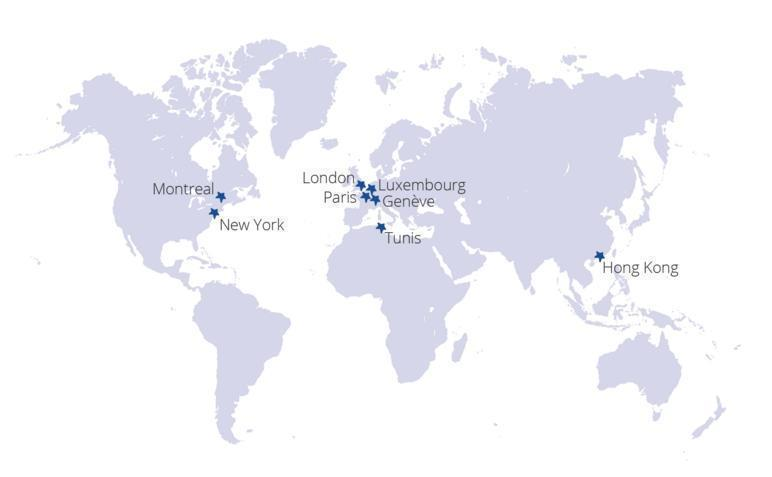
\includegraphics[scale=0.6]{img/talan1.jpg}
\centering
\caption{Implantation de Talan dans le monde}
\label{fig:talan-monde}
\end{figure}
%%%%%%%%%%%%%%%%%%%%%%%%%%%%%%%%%%%%%%%%%%%%%%%%%%%%%%%%%%%%%%%%
\subsubsection{Secteurs d’activité}
Talan Tunisie couvre essentiellement :
\begin{itemize}
\item[•]  Le secteur de la finance à travers une collaboration avec des banques d’investissement et des sociétés d'assurances.
\item[•] Le secteur de la télécommunication à travers des projets destinés aux opérateurs télécom et un ensemble de fournisseurs d’accès à internet.
\item[•] Le secteur du transport et de la logistique.
\item[•] Le secteur de l’énergie à travers des projets de développement visant des opérateurs de services liés à l’électricité,au gaz,à l'eau, etc.
\end{itemize}
%%%%%%%%%%%%%%%%%%%%%%%%%%%%%%%%%%%%%%%%%%%%%%%%%%%%%%%%%%%%%%%%%
%\color{red}
\subsection{Contexte du projet}
%\color{red} Présenter un peut qu'est ce qu'un système ERP et son inmportance dans une entreprise puis mentionne que Talan utilise Byblos comme outil ERP \\\color{black}
Les entreprises utilisent un système \textbf{"Enterprise Ressource Planning"} (ERP) en tant que progiciel permettant la gestion de l’ensemble des processus opérationnels d’une entreprise en intégrant plusieurs modules de gestion : module RH, module de gestion des fournisseurs, module de gestion de la comptabilité$\dots$\\ 
Autrement dit, l’ERP représente la « colonne vertébrale » d’une entreprise. \textbf{Talan Tunisie} a fait le choix d’investir dans la refonte de son système ERP, appellé \textbf{BYBLOS}, dont nous allons présenter la version existante. Nous exposerons aussi ses limites et l'impact de son architecture monolithique pour justifier la migration vers une architecture microservices.
%%%%%%%%%%%%%%%%%%%%%%%%%%%%%%%%%%%%%%%%%%%%%%%%%%%%%%%%%%%
\subsubsection{Présentation de l'outil BYBLOS}
BYBLOS est un ERP développé par les équipes de Talan Tunisie consulting, contenant plusieurs modules à savoir:
%\color{red} \\Tu peux mettre ici une figure d'acceuil de l'outil.\\
%Explique le but de chaque module en une phrase comme celui de gestion de fournisseurs.
\color{black}
\begin{itemize}
    \item Un module de gestion des ressources humaines : qui gère les fiches RH du personnel, ainsi que les soldes de congés.
    \item Un module de gestion des candidats : qui gère les fiches des candidats et leurs entretiens.
    \item Un module de gestion des collaborateurs : qui gère les fiches des collaborateurs.
    \item Un module de gestion des fournisseurs: qui gère les données personnelles et la situation des fournisseurs.
    \item Un module de gestion des contrats : qui expose le type de contrats et leurs détails (date d'effet, date de fin, durée $\dots{}$).
    
\end{itemize}
Dans le cadre de ce projet, nous nous intéressons au module de \textbf{gestion des candidats}.
Cette solution existante, basée sur une architecture monolithique, est développée avec Java Entreprise Edition (JEE) et Java Server Faces (JSF).
%\color{red} \\Mentionnes que dans ton projet tu t'intéresses au module de gestion des candidats\color{black}
%\subsubsection{Problématique: Impact de l’architecture monolithique sur l’outil Byblos}
%en effet, la solution existante de Byblos présente plusieurs limites :
%\begin{itemize}
    %\item  Le fait que Byblos est constitué en un seul Bloc, à chaque modification, l'équipe opérationnelle doit redéployer toute l'application et donc il faut refaire les tests(test unitaire, test de régression et test fonctionnel) et la révision de la qualité du code de tout le projet.
    %\item le nombre énorme de classes et les milliers de lignes de code ajoutés à chaque modification, augmentent la complexité du projet et rend l'application nécessite plus de ressources matérielles ce qui est très coûteux.
    %\item A chaque fois où un nouveau développeur intègre l'équipe de développement, il lui faut plusieurs jours voir semaines pour comprendre le code.
%\end{itemize}
%\newpage
%%%%%%%%%%%%%%%%%%%%%%%%%%%%%%%%%%%%%%%%%%%%%%%%%%%%%%%%%%%
\section{Problématique}
%\color{red}Ajoutes une phrase introductive ici.
\color{black}Dans cette section, nous allons présenter l'architecture monolithique, ainsi que son impact sur l'outil BYBLOS. 
%En fin nous proposerons la solution.
%%%%%%%%%%%%%%%%%%%%%%%%%%%%%%%%%%%%%%%%%%%%%%%%%%%%%%%%%%%
%\subsection{Les architectures monolithiques}
%\color{red}Définis ici qu'est ce qu'une architecture monolithique (utilises des figures si c possible). Dans la sous-section suivante tu vas lister ses inconvénients majeurs et leur impact sur Byblos.
\color{black}
L'architecture monolithique est l'architecture traditionnelle où  toutes les tâches sont réalisées dans une seule et grande application. Tous les services individuels accèdent à une grande base de données et sont édités via une interface utilisateur, tous implémentés dans une seule application. 
\begin{figure}[H]
    \centering
    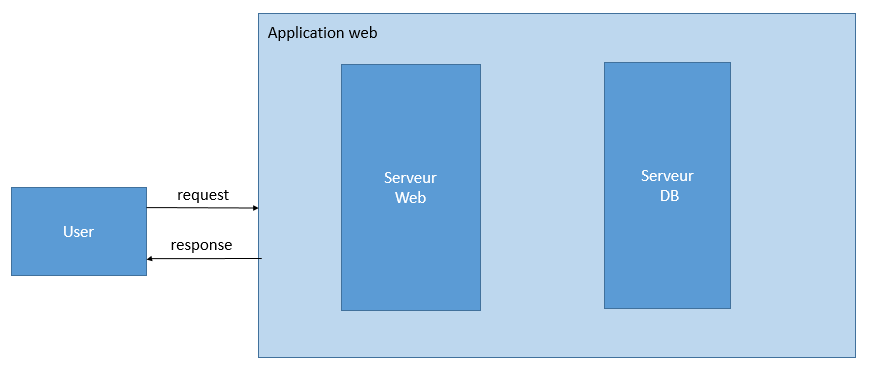
\includegraphics[scale=0.5]{img/archi mono.PNG}
    \caption{Architecture monolithique}
    \label{fig:Architecture monolitique}
\end{figure}

\color{black}
%\subsection{Impact de l’architecture monolithique sur l’outil Byblos}
Une architecture monolithique représente le modèle traditionnel unifié de conception d'un programme informatique. En se basant sur une telle architecture, la maintenance de l'outil BYBLOS est devenue trop difficile à cause de la complexité de l'application qui augmente à chaque itération.
%se base sur, rend la maintenance ou l'ajout d'un nouveau module très difficile due à la complexité du projet qui augmente à chaque itération.


%De plus, Le choix des technologies est décidé avant que le développement de l’application commence. Ainsi qu'une seule technologie est utilisée pour le développement de l’application.
En outre, une légère modification apportée à une petite partie de l’application nécessite la construction et le déploiement d'une version entièrement nouvelle et requiert une durée des tests automatiques et des builds plus longue, ce qui engendre un coût supplémentaire. De plus, l'application est constituée d'un seul bloc, un dysfonctionnement sur une partie du système affecte toute l’application. Cette architecture réduit l'agilité de l’équipe et la fréquence de livraison à cause du fort couplage entre les composants de l'application.\\
L'outil BYBLOS est une application web composée de trois couches comme le montre la Figure \ref{fig:architecure BYBLOS existante} :
\begin{itemize}
    \item \textbf{Couche présentation} : cette couche est composée des pages JSF et des servlets.
    \item \textbf{Couche métier} : cette couche représente l’ensemble métier de l’application. Elle est composée des EJBs.
    \item \textbf{Couche persistance} : c'est la couche Data Access Objects (DAO) qui transforme les objets métiers en données sérialisées, et inversement pour les échanges avec la base de donnée PostgreSql. Elle est réalisée en se basant sur le framework Hibernate/JPA.
\end{itemize}
\begin{figure}[H]
    \centering
    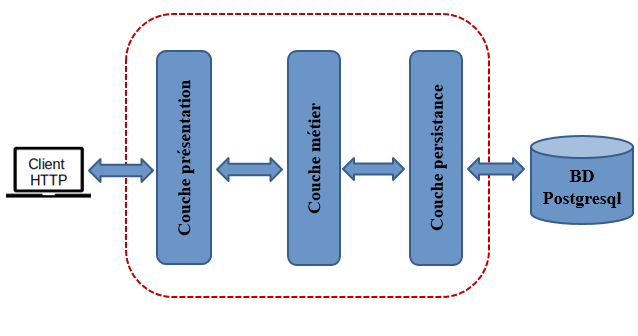
\includegraphics[scale=0.8]{img/archi mono byblos.PNG}
    \caption{Architecture monolithique de BYBLOS}
    \label{fig:architecure BYBLOS existante}
\end{figure}
% \begin{figure}[H]
%     \centering
%     \includegraphics[scale=0.5]{img/archit-mono.png}
%     \caption{Architecture monolithique de BYBLOS}
%     \label{fig:byblos_exist}
% \end{figure}
%%%%%%%%%%%%%%%%%%%%%%%%%%%%%%%%%%%%%%%%%%%%%%%%%%%%%%%%%%%%%%%%
\section{Solution proposée: Migration vers une architecture microservices}
\textbf{Talan} prévoit de renforcer son effectif d’ici fin 2020 en intégrant 3000 nouveaux collaborateurs et d’ouvrir, dès septembre 2020, un siège international à Londres ainsi que des bureaux à l’étranger, notamment en Belgique, en Italie et aux Pays-Bas.\\
De ce fait, le module de gestion des candidats dans l'ERP BYBLOS doit être disponible et performant à cette période. Après une étude approfondie de la solution existante, et dans le but de surmonter les limites de l'architecture monolithique ainsi que dans un souci de performance, l'équipe BYBLOS a décidé de faire une refonte de l'ERP BYBLOS existant vers une architecture microservices tout en améliorant les IHMs.\\
C'est dans ce cadre que s'inscrit notre projet de fin d'études, qui consiste à réaliser la migration du module de gestion des candidats de la solution existante vers une architecture microservices.\\
Notre travail consiste donc à :
\begin{itemize}
    \item Concevoir et implémenter le microservice de gestion des candidats;
    \item Enregistrer le microservice dans le  serveur de découverte (Eureka) et dans le Gateway (zuul);
    \item Ajouter le fichier de configuration du microservice dans le serveur de configuration.  
\end{itemize}
  
\color{black}
%%%%%%%%%%%%%%%%%%%%%%%%%%%%%%%%%%%%%%%%%%%%%%%%%%%%%%%%%%%%%%%
\section{Architecture microservices}

%\color{red}Ajoutes une phrase introductive ici
\color{black}
Dans cette section, nous définirons l'architecture microservices. Par la suite, nous allons présenter les caractéristiques d'un microservice, et enfin les avantages de cette architecture par rapport à l'architecture monolithique comme le montre la figure \ref{fig:architecture micro vs architecture mono}. \\
%\subsection{L'architecture microservices}
\begin{figure}[H]
    \centering
    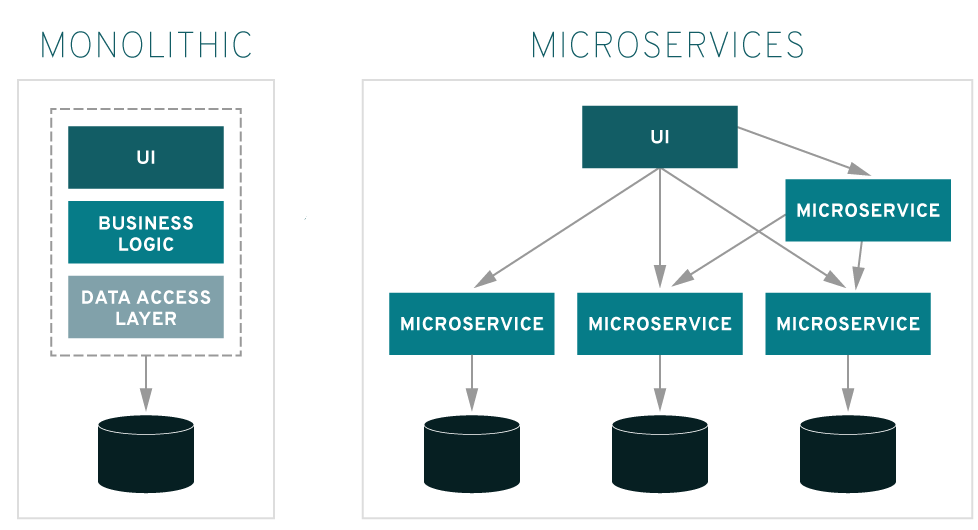
\includegraphics[scale=0.6]{img/monolithic-vs-microservices.png}
    \caption{Comparaison entre les architectures microservices et monolithique}
    \label{fig:architecture micro vs architecture mono}
\end{figure}

L'architecture microservices est une méthode distinctive de développement des systèmes logiciels, qui a connu une popularité grandissante ces dernières années. Il s'agit d'une méthode de développement d'applications logicielles en tant que suite de services modulables et indépendants.\\
Ce style d’architecture présente plusieurs avantages comme l’hétérogénéité technologique, la résistance contre l’échec, la scalabilité sur mesure, la facilité de déploiement, l’alignement organisationnel et la réutilisabilité.
%%%%%%%%%%%%%%%%%%%%%%%%%%%%%%%%%%%%%%%%%%%%%%%%%%%%%%%%%%%%%%%%
\subsection{Caractéristiques d'un microservice}
L’architecture microservices possède plusieurs caractéristiques qu’il est essentiel d’appliquer durant la conception et le développement d’une application basée sur les microservices.
\begin{enumerate}
    \item[1] \textbf{Concentration sur une seule fonctionnalité:}  Un microservice implémente une seule fonctionnalité dont il est responsable dans tout le système. Une fonctionnalité peut être une fonctionnalité métier contribuant à l’objectif du système, ou une fonctionnalité technique utilisée par plusieurs fonctionnalités métier.
    \item[2] \textbf{Déploiement individuel des microservices:} Chaque microservice doit être déployable indépendamment des autres. Ce point est important : tout changement ou mise à jour d'un microservice doivent être réalisés sans toucher aux autres microservices ni affecter leur exécution.\\
    Le système doit continuer à fonctionner correctement durant la mise à jour du microservice en question, ainsi qu'après l’avoir redéployé.
    \item[3] \textbf{Indépendance des microservices:} Un microservice peut correspondre à un ou plusieurs processus. Il doit être obligatoirement hébergé sur des processus indépendants. En d’autres termes, il ne doit pas partager un processus avec un autre microservice.\\
    En revanche, il peut être constitué de plusieurs processus, notamment dans le cas d'un accès à une base de données. Autrement dit, seul ce service peut accéder à cette base de données. C’est une façon d’éviter au maximum les interdépendances entre les microservices.\\
    Par exemple si on développe deux microservices sur le même processus, nous risquons d’avoir des interdépendances qui vont conduire à l’obligation de déployer les deux en même temps, ce qui est contradictoire avec les caractéristiques des microservices.
    \item[4] \textbf{Taille des microservices:} Comme l’indique le nom ”micro”, les microservices doivent être concentrés sur une seule et unique fonctionnalité, de façon à ce que leur développement et leur maintenance puisse se faire par des équipes de petites tailles.
    \item[5] \textbf{Remplaçabilité:} On doit pouvoir remplacer n’importe quel microservice du système dans un temps raisonnablement court.
    \item[6] \textbf{Conception pour l’échec:} L’un des atouts majeurs des microservices est qu’ils sont conçus pour être tolérants aux pannes. Dans une application en microservices, si un service échoue, les autres services ne sont pas affectés et adaptent leurs fonctionnements selon l’état du système dans lequel ils évoluent.
\end{enumerate}
%%%%%%%%%%%%%%%%%%%%%%%%%%%%%%%%%%%%%%%%%%%%%%%%%%%%%%%%%%%%%%%%
\subsection{Architecture monolithique Vs microservices}

Le tableau \ref{tab:comp} ci-dessous présente les principales différences entre les architectures microservice et monolithique.
\begin{longtable}[c]{
    |p{.20\textwidth}|
    |p{.35\textwidth}|
    |p{.35\textwidth}|
}
    \hline
    &    \textbf{Architecture Microservice}
    &    \textbf{Architecture Monolithique}\\
    \hline
    \textbf{Mise sur le marché}
    & Déploiement et mises à jour en microservices sont plus rapides et plus agiles.
    &Déploiement et mises à jour en un seul bloc, nécessitent plus de temps et sont moins agiles.    \\
    \hline
     \textbf{Haute évolutivité}
    & La possibilité d'étendre les déploiements sur plusieurs serveurs et infrastructures.
    &Le déploiement se fait sur un seul serveur.\\
    \hline
     \textbf{Résilience}
    & Les microservices sont indépandants. Lorsqu'un service tombe en panne, l'ensemble de l'application continue à fonctionner.
    & Lorsqu'un module tombe en panne, l'intégralité de l'application cesse de fonctionner.\\
    \hline
    \textbf{Facilité de déploiement}
    & Les applications basées sur des microservices sont plus modulaires et légères.
    &Les applications monolithiques sont déployées en un seul bloc et sont plus lourdes.\\
    \hline
    \textbf{Ouverture}
    & Les développeurs ont la liberté de choisir la technologie et le langage qui leur conviennent le mieux pour chaque fonction.
    &Les développeurs ne peuvent utiliser qu'une seule technologie et un seul langage pour toute l'application.\\
    \hline
\caption{Architecture microservices Vs monolithique}
\label{tab:comp}
\end{longtable} 
% \begin{itemize}
%     \item[-] \textbf{Mise sur le marché plus rapide}\\
% Comme les cycles de développement sont plus courts, l'architecture de microservices permet des déploiements et mises à jour plus agiles.
%     \item[-] \textbf{Haute évolutivité}\\
% À mesure que la demande pour certains services augmente, vous pouvez étendre les déploiements sur plusieurs serveurs et infrastructures pour répondre à vos besoins.
%     \item[-] \textbf{Résilience}\\
% Lorsqu'ils sont développés correctement, ces services indépendants n'ont aucun impact les uns sur les autres. Cela signifie que, lorsqu'un élément tombe en panne, l'ensemble de l'application ne cesse pas de fonctionner comme c'est le cas avec le modèle monolithique.
%     \item[-] \textbf{Facilité de déploiement}\\
% Les applications basées sur des microservices sont plus modulaires et légères que les applications monolithiques classiques. Aussi, vous pouvez les déployer plus sereinement. Certes, cela requiert une meilleure coordination, mais les bénéfices peuvent être énormes.
%     \item[-] \textbf{Accessibilité}\\
% Vu que l'application est décomposée en plusieurs éléments, les développeurs peuvent plus facilement comprendre, mettre à jour et améliorer chacun de ces éléments. Résultat : des cycles de développement plus courts, surtout s'ils sont associés à des méthodes de développement agiles.
%     \item[-] \textbf{Ouverture}\\
% Grâce aux API qui utilisent plusieurs langages, les développeurs ont la liberté de choisir la technologie et le langage qui conviennent le mieux à chaque fonction.
% \end{itemize}
%%%%%%%%%%%%%%%%%%%%%%%%%%%%%%%%%%%%%%%%%%%%%%%%%%%%%%%%%%%%%%%%
\section{Méthodologie de développement adoptée: Scrum}
Le choix de la méthodologie à utiliser durant le développement d'un logiciel doit répondre aux critères suivants :
\begin{itemize}
    \item[•] Exprimer au mieux les besoins des futurs clients.
    \item[•] Permettre de développer une application robuste et évolutive.
    \item[•] Élaborer une application qui répond aux besoins des clients dans des délais respectables.
\end{itemize}
Nous avons travaillé avec la méthode Scrum, déjà utilisée par l’équipe BYBLOS. Nous présentons, dans la suite, la méthode Scrum, les différents intervenants dans notre projet ainsi que son cycle de vie.
\subsection{Présentation de la méthode SCRUM}
Scrum est une méthode qui implémente les bonnes pratiques du Manifeste Agile dont l'utilisation s’étend au-delà du domaine informatique. Elle vise à produire les meilleurs logiciels possibles, le plus rapidement possible. Le cycle d'un projet Scrum est illustré dans la Figure  \ref{fig:scrum}.
\begin{figure}[H]
\centering
\frame{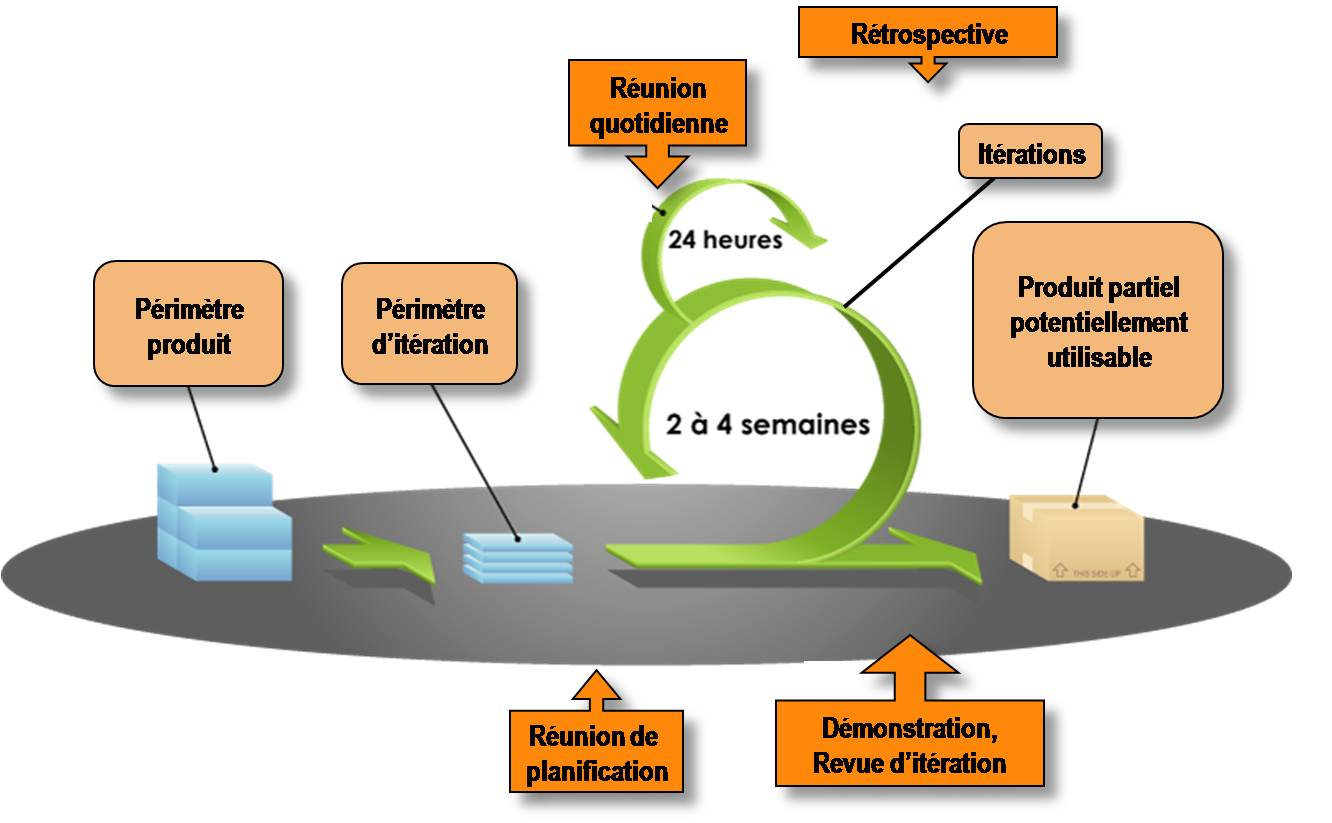
\includegraphics[scale=0.65]{img/cycle-scrum.jpg}}
\caption{Cycle de vie de SCRUM}
\label{fig:scrum}
\end{figure}
%%%%%%%%%%%%%%%%%%%%%%%%%%%%%%%%%%%%%%%%%%%%%%%%%%%%%%%%%%%%%%%
\subsection{Les rôles dans SCRUM}
La méthodologie SCRUM fait intervenir trois rôles principaux qui sont :
\begin{itemize}
    \item \textbf{Le Scrum Master:} C’est le coach de l’équipe, il assure plusieurs tâches : 
    \begin{itemize}
    \item Assister l’équipe pour appliquer la philosophie et les pratiques de Scrum.
    \item S’assurer que l’équipe bénéficie des meilleures conditions pour accomplir les tâches nécessaires.
    \item Surmonter les obstacles éventuels: prendre en compte les problèmes qui surviennent à tout moment sur le projet pour les éliminer.
    \item Faire en sorte que l’équipe reste concentrée sur le véritable objectif du projet, en s’assurant que chacun participe pleinement aux travaux de l’équipe.
\end{itemize}
    \item \textbf{Le Product Owner:} Il est le propriétaire du \textbf{Product Backlog}. Il représente les utilisateurs et est fortement impliqué dans les réunions de planification et d’avancement. Il a aussi la capacité d’annuler le sprint avant échéance.
    \item \textbf{La Scrum Team:} Il s’agit de l’équipe de développement. Elle produit chaque itération du projet, et ses membres sont les mêmes tout au long du projet.
\end{itemize}
%%%%%%%%%%%%%%%%%%%%%%%%%%%%%%%%%%%%%%%%%%%%%%%%%%%%%%%%%%%%%%%%
\subsection{Cycle de vie de Scrum}

\begin{itemize}
    \item [•]\textbf{ Backlog produit} : lister toutes les fonctionnalités en les triant par priorité.
    \begin{itemize}
    \item Besoins priorisés par le product owner. 
    \item Besoins évalués par l’équipe.
\end{itemize}
    \item [•] \textbf{Backlog de sprint} : extraire les fonctionnalités qui vont être développées au prochain sprint.
    \begin{itemize}
    \item Extrait du backlog produit.
    \item Besoins éclatés en tâches.
\end{itemize}
    \item [•] \textbf{Sprint} : la scrum team commence à developper les fonctionnalités du Sprint
    \begin{itemize}
    \item Développement des fonctionnalités du backlog de sprint. 
    \item Aucune modification du backlog de sprint possible.
\end{itemize}
    \item [•] \textbf{Mêlée quotidienne} : une petite réunion journalière pour identifier les problèmes rencontrés par chaque membre de l'équipe de développement.
    \begin{itemize}
    \item Point de contrôle quotidien de l’équipe. 
    \item Interventions régulées : 2 minutes par personne.
\end{itemize}
    \item [•] \textbf{Incrément logiciel} : Après avoir achevé le sprint et testé les fonctionnalités, un livrable est prêt à être déployé. 
    \begin{itemize}
    \item Livrable remis au Product Owner à la fin du sprint. 
\end{itemize}
\end{itemize}


\section*{Conclusion}
Dans ce chapitre, nous avons défini le cadre général de notre projet, en présentant l'organisme d'accueil et la solution proposée. Nous avons aussi défini les principales notions qui constituent la base de ce travail. Le prochain chapitre sera consacré à la spécification des besoins fonctionnels et non-fonctionnels de notre système.